\section{Design}
\label{s:gen}

This section describes \sys's design for constraint generation and
solving.

\subsection{Basic Architecture}

\sys's constraint generator is implemented as a set of compiler
passes in the LLVM~\cite{lattner:llvm} framework.  The workflow is
shown in \autoref{f:flow}.  The error and path constraint generation
passes work on LLVM intermediate representations, which are compiled
from source code with all optimizations turned off.  They inspect
one function at a time, so as to bound the size of constraints.

To improve the accuracy, \sys allows users to annotate the ranges
of variables, such as function parameters and structure fields, as
additional constraints. It also employs a whole-program pass that
infers the range constraints across the call graph.

\begin{figure}
\centering
\resizebox{0.9\linewidth}{!}{
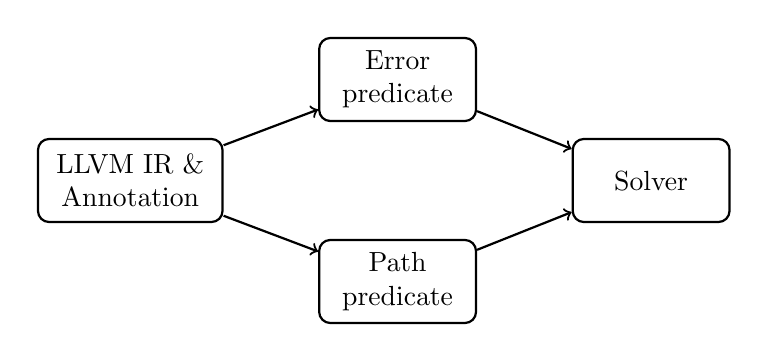
\begin{tikzpicture}[
	block/.style={
		rectangle, rounded corners,
		draw=black, thick,
		text width=5em, minimum height=3em, text centered
	},
	line/.style={draw, thick, ->},
	]
	\matrix[row sep=2mm, column sep=12mm] {
		& \node [block] (ec) {Error predicate}; & \\
		\node [block, text width=6em] (ir) {LLVM IR \& Annotation};
		&
		& \node [block] (sol) {Solver}; \\
		& \node [block] (pc) {Path predicate}; & \\
	};

	\path [line] (ir) -- (ec);
	\path [line] (ir) -- (pc);
	\path [line] (ec) -- (sol);
	\path [line] (pc) -- (sol);
\end{tikzpicture}

}
\caption{\sys's workflow.}
\label{f:flow}
\end{figure}

\subsection{Transformations}

Pointer arithmetic simplification.
- symbolic~\cite{engelen:symbolic}.

Integer operation sinking.

Checking idiom recognition.

\paragraph{Value equality testing.}
How to determine the values from two load instructions
are the same? Load hoisting, unsound aliasing rules.

\autoref{f:hoist} shows in the hoisting algorithm.

\begin{figure}
\begin{algorithmic}
\footnotesize
\Procedure{Hoist}{$I$}\Comment{$I$ is a load instruction}
\State $\mathit{loc} \gets I$'s memory location to load from
\Loop
\If{\textbf{not} \Call{HoistInBlock}{$I$, $\mathit{loc}$}}
	\State \Return
\EndIf
\State $\mathit{blk} \gets$ \Call{ChooseTargetBlock}{$I$, $\mathit{loc}$}
\If{$\mathit{blk} = \textbf{nil}$}
	\State \Return
\EndIf
\State Move $I$ to the end of $blk$
\EndLoop
\EndProcedure
\\
\Function{HoistInBlock}{$I$, $\mathit{loc}$}
\Loop
\State $\mathit{prev} \gets I$'s previous instruction in current block
\If{$\mathit{prev} = \textbf{nil}$}
	\Comment{Moved to beginning of the block?}
	\State \Return \textbf{true}
\EndIf
\If{$\mathit{prev}$ may modify $\mathit{loc}$ \textbf{or} \\
\hspace{3.6em} \textbf{not} $\mathit{loc}$ dominates $\mathit{prev}$}
	\State \Return \textbf{false}
\EndIf
\State Move $I$ before $\mathit{prev}$
\EndLoop
\EndFunction
\\
\Function{ChooseTargetBlock}{$I$, $\mathit{loc}$}
\State $\mathit{blk} \gets I$'s block
\State $\mathit{anc} \gets$ the common ancestor of $\mathit{blk}$'s predecessor(s)
\If{$\mathit{anc} = \mathit{blk}$ \textbf{or} \textbf{not} $\mathit{loc}$ dominates $\mathit{anc}$}
	\State \Return \textbf{nil}
\EndIf
\State $\mathit{blkset} \gets \{\mathit{anc}\}$
\If{\Call{CanBlocksModify}{$\mathit{loc}$, $blk$, $\mathit{blkset}$}}
	\State \Return \textbf{nil}
\EndIf
\State \Return $\mathit{anc}$
\EndFunction
\\
\Function{CanBlocksModify}{$\mathit{loc}$, $\mathit{blk}$, $\mathit{blkset}$}
\ForAll{$b \in \mathit{blk}$'s predecessor(s)}
	\If{$b \notin \mathit{blkset}$}
		\State $\mathit{blkset} \gets \mathit{blkset} \cup \{b\}$
		\ForAll{$\mathit{instr} \in b$}
			\Comment{Can $b$ modify $\mathit{loc}$?}
			\If{$\mathit{instr}$ may modify $\mathit{loc}$}
				\State \Return \textbf{true}
			\EndIf
		\EndFor
		\If{\Call{CanBlocksModify}{$\mathit{loc}$, $b$, $\mathit{blkset}$}}
			\State \Return \textbf{true}
		\EndIf
	\EndIf
\EndFor
\State \Return \textbf{false}
\EndFunction

\end{algorithmic}

\caption{The hoisting algorithm to move a load instruction to the
earliest possible point in a control-flow graph.  It repeats the
two phases: first try to move the instruction to the beginning of
its basic block; if successful, try to move it into the common
ancestor of the block's predecessors.}
\label{f:hoist}
\end{figure}

\subsection{Error Constraint Generation}

\paragraph{Conversion constraint.}
\sys by default does not generate constraints for checking integer
conversions.  One may simply invoke GCC with \cc{-Wconversion} to
inspect potentially dangerous conversions.
[[[\sys does something for critical integers, array indices, annotated sizes.]]]

\paragraph{In-loop constraint.}
Move in-loop constraints out.

\subsection{Path Constraint Generation}

Path constraint generation.

unroll loops once.

\subsection{Value Range Inference}

Range constraint \& annotations?

\subsection{Limitations}

miss bugs in some configurations, architectures,
and assembly code.
